\documentclass[
11pt, % The default document font size, options: 10pt, 11pt, 12pt
%codirector, % Uncomment to add a codirector to the title page
]{charter} 


% El títulos de la memoria, se usa en la carátula y se puede usar el cualquier lugar del documento con el comando \ttitle
\titulo{Reconocimiento de eventos quirúrgicos a través de visión por computadora} 

% Nombre del posgrado, se usa en la carátula y se puede usar el cualquier lugar del documento con el comando \degreename
\posgrado{Maestría en Computación de Borde} 
%\posgrado{Carrera de Especialización en Internet de las Cosas} 
%\posgrado{Carrera de Especialización en Inteligencia Artificial}
%\posgrado{Maestría en Sistemas Embebidos} 
%\posgrado{Maestría en Internet de las cosas}

% Tu nombre, se puede usar el cualquier lugar del documento con el comando \authorname
% IMPORTANTE: no omitir titulaciones ni tildación en los nombres, también se recomienda escribir los nombres completos (tal cual los tienen en su documento)
\autor{Esp. Ing. Marín A. Brocca}

% El nombre del director y co-director, se puede usar el cualquier lugar del documento con el comando \supname y \cosupname y \pertesupname y \pertecosupname
\director{Dr. Ing. Axel Soto}
\pertenenciaDirector{UNS-CONICET} 
\codirector{Dr. Ing. Felix Sebastian Leo Thomsen} % para que aparezca en la portada se debe descomentar la opción codirector en los parámetros de documentclass
\pertenenciaCoDirector{UNS}

% Nombre del cliente, quien va a aprobar los resultados del proyecto, se puede usar con el comando \clientename y \empclientename
\cliente{Luciano Torun}
\empresaCliente{Wúru}
 
\fechaINICIO{24 de junio de 2025}		%Fecha de inicio de la cursada de GdP \fechaInicioName
\fechaFINALPlan{19 de agosto de 2025} 	%Fecha de final de cursada de GdP
\fechaFINALTrabajo{abril de 2026}	%Fecha de defensa pública del trabajo final


\begin{document}

\maketitle
\thispagestyle{empty}
\pagebreak


\thispagestyle{empty}
{\setlength{\parskip}{0pt}
\tableofcontents{}
}
\pagebreak


\section*{Registros de cambios}
\label{sec:registro}


\begin{table}[ht]
\label{tab:registro}
\centering
\begin{tabularx}{\linewidth}{@{}|c|X|c|@{}}
\hline
\rowcolor[HTML]{C0C0C0} 
Revisión & \multicolumn{1}{c|}{\cellcolor[HTML]{C0C0C0}Detalles de los cambios realizados} & Fecha      \\ \hline
0      & Creación del documento                                 &\fechaInicioName \\ \hline
1      & Se completa hasta el punto 9 inclusive                & 7 de julio de 2025\\ \hline
2      & Se completa hasta el punto 10 inclusive	& 15 de julio de 2025 \\ \hline
%		  Se puede agregar algo más \newline
%		  En distintas líneas \newline
%		  Así                                                    & {día} de {mes} de 202X \\ \hline
%3      & Se completa hasta el punto 12 inclusive                & {día} de {mes} de 202X \\ \hline
%4      & Se completa el plan	                                 & {día} de {mes} de 202X \\ \hline

% Si hay más correcciones pasada la versión 4 también se deben especificar acá

\end{tabularx}
\end{table}

\pagebreak



\section*{Acta de constitución del proyecto}
\label{sec:acta}

\begin{flushright}
Buenos Aires, \fechaInicioName
\end{flushright}

\vspace{2cm}

Por medio de la presente se acuerda con el \authorname\hspace{1px} que su Trabajo Final de la \degreename\hspace{1px} se titulará ``\ttitle'' y consistirá en la creación de un modelo de una aplicación basada en inteligencia artificial para la identificación de eventos en quirófanos por medio de visión por computadora. El trabajo tendrá un presupuesto preliminar estimado de 700 horas y un costo estimado de \$ 4000, con fecha de inicio el \fechaInicioName\hspace{1px} y fecha de presentación pública en el mes de  \fechaFinalName.

Se adjunta a esta acta la planificación inicial.

\vfill

% Esta parte se construye sola con la información que hayan cargado en el preámbulo del documento y no debe modificarla
\begin{table}[ht]
\centering
\begin{tabular}{ccc}
\begin{tabular}[c]{@{}c@{}}Dr. Ing. Ariel Lutenberg \\ Director posgrado FIUBA\end{tabular} & \hspace{2cm} & \begin{tabular}[c]{@{}c@{}}\clientename \\ \empclientename \end{tabular} \vspace{2.5cm} \\ 
\multicolumn{3}{c}{\begin{tabular}[c]{@{}c@{}} \supname \\ Director del Trabajo Final\end{tabular}} \vspace{2.5cm} \\
\end{tabular}
\end{table}

\section{1. Descripción técnica-conceptual del proyecto a realizar}
\label{sec:descripcion}

El presente proyecto se realiza en el marco del programa de vinculación con Wúru, empresa fundada en 2019 por un equipo con profunda experiencia en entornos hospitalarios que emergió con la visión de mejorar la eficiencia operativa en instituciones de salud. El foco de este equipo es la optimización continua de procesos mediante la capitalización del vasto volumen de datos generados por sistemas de registros médicos electrónicos (EMR) y equipos radiológicos. En función de esto, la empresa identificó desafíos críticos en el área quirúrgica: el alto costo asociado al tiempo ocioso de los quirófanos y la falta de precisión en el registro de eventos clave,  que impactan directamente en la planificación y utilización de recursos.

El problema central que se busca abordar radica en la naturaleza manual y propensa a errores de la documentación de eventos en las salas de operaciones. Actualmente, y dependiendo del sistema EMR empleado, tareas como el inicio y fin de una cirugía, la entrada o salida de pacientes o la limpieza de la sala dependen de la intervención manual del personal de enfermería. Esta dependencia no solo introduce inconsistencias y omisiones en los datos, sino que también genera una carga administrativa adicional y puede llevar a la duplicación de esfuerzos en diferentes sistemas. La consecuencia directa es el desaprovechamiento de los recursos del quirófano, un aumento en los costos operativos y una visibilidad limitada sobre el flujo real de trabajo. En la figura \ref{fig:lifecycle} se ejemplifica el ciclo de uso de un quirófano.

\begin{figure}[htpb]
	\centering 
	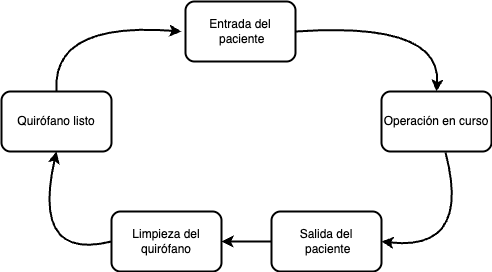
\includegraphics[width=.6\textwidth]{./Figuras/lifecycle.png}
	\caption{Ciclo de preparación y uso del quirófano.}
	\label{fig:lifecycle}
\end{figure}

En el mercado de soluciones hospitalarias existen diferentes alternativas que emplean en mayor o menor medida sistemas de grabaciones de video y voz con diferentes propósitos, como puede ser el monitoreo de eventos intraoperatorios, por ejemplo sangrado, conteo automático del instrumental empleado o capacitaciones a nuevo personal. Los principales inconvenientes de estas aplicaciones son su naturaleza cerrada, es decir, su limitada capacidad para ser integradas a sistemas locales, y el riesgo de dependencia del proveedor (\textit{vendor lock-in}).

Para resolver estos problemas se deben sortear los desafíos que incluyen la gestión del gran volumen de datos de video, la complejidad del etiquetado de eventos temporales (considerando variaciones de iluminación y perspectivas), el desarrollo de un modelo robusto capaz de generalizar a diversas condiciones de quirófano, y la construcción de una aplicación de demostración que refleje fielmente el potencial de la solución.

En la figura \ref{fig:Esquema} se presenta el diagrama en bloques del sistema propuesto. Se observa que la solución se fundamenta en la ingesta de videos provenientes de cámaras de vigilancia instaladas en las salas de operaciones. Estos videos son procesados por un modelo de visión por computadora entrenado para identificar eventos específicos como actividades de limpieza, el desarrollo de una operación y la entrada o salida de pacientes. A partir de esto, el sistema genera una salida estructurada que refleja el estado actual del quirófano. Dicha información se almacena en una base de datos operacional que alimenta una aplicación de demostración. Esta permite visualizar el estado del quirófano por medio de una interfaz intuitiva para la monitorización y la toma de decisiones operativas.

\begin{figure}[htpb]
	\centering 
	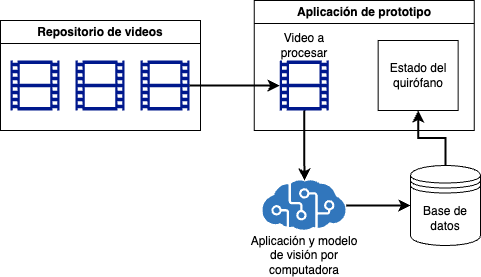
\includegraphics[width=.6\textwidth]{./Figuras/CEIA-GDP-Esquema.png}
	\caption{Diagrama en bloques del sistema a desarrollar.}
	\label{fig:Esquema}
\end{figure}

\section{2. Identificación y análisis de los interesados}
\label{sec:interesados}

\begin{table}[ht]
%\caption{Identificación de los interesados}
%\label{tab:interesados}
\begin{tabularx}{\linewidth}{@{}|l|X|X|l|@{}}
\hline
\rowcolor[HTML]{C0C0C0} 
Rol           & Nombre y Apellido & Organización 	& Puesto 	\\ \hline
Auspiciante       & \clientename      &\empclientename	&        CEO	\\ \hline
Cliente       & \clientename      &\empclientename	&        CEO	\\ \hline
Responsable   & \authorname       & FIUBA        	& Alumno 	\\ \hline
Colaborador       & Javier Roberts      &\empclientename	&        CTO	\\ \hline
Orientador    & \supname	      & \pertesupname 	& Director del Trabajo Final \\ \hline
Opositores    &    Aún no conocidos               &        -      	&        -	\\ \hline
Usuario final & Usuarios de la plataforma de gestión hospitalaria Wúru. & - & - \\ \hline

\end{tabularx}
\end{table}


\section{3. Propósito del proyecto}
\label{sec:proposito}

Desarrollar un prototipo de aplicación que, por medio de técnicas de visión por computadora, permita la automatización de los procesos asociados a la gestión de quirófanos.



\section{4. Alcance del proyecto}
\label{sec:alcance}

El proyecto incluye:
\begin{itemize}
	\item Relevamiento detallado de los requerimientos del cliente.
	\item Armado del dataset a partir de los datos crudos entregados por el cliente.
	\item Planteo de la tarea de visión por computadora a ser utilizada. 
	\item Selección, entrenamiento y ensayos con modelos de inteligencia artificial.
	\item Procesamiento del dataset.
	\item Desarrollo de un prototipo de aplicación de tres capas (backend, frontend y base de datos).
	\item Desarrollo de APIs para la integración entre la aplicación y el modelo.
	\item Ejecución de pruebas funcionales y de integración.
	\item Documentación y entrega de recomendaciones al cliente.
	\item Escritura de la memoria del trabajo final y defensa ante jurados.
	
\end{itemize}

Los siguientes elementos quedan fuera del alcance:
\begin{itemize}
	\item Implementación del sistema en producción.
	\item Integración del modelo con las aplicaciones del cliente.
	\item Integración de la aplicación con los sistemas de cámaras en los quirófanos. 

\end{itemize}



\section{5. Supuestos del proyecto}
\label{sec:supuestos}

Para el desarrollo del presente proyecto se supone que: 

\begin{itemize}
	\item Se dispondrá de la suficiente cantidad de videos para el correcto procesamiento e identificación de eventos..
	\item La calidad de los videos será la adecuada para su procesamiento.
	\item En caso de ser necesario, se contará con la ayuda de recursos por parte del cliente para el procesamiento y entrenamiento del modelo.
	\item Se dispondrá de materiales y/o de soporte académico para completar el proyecto.
	\item Se contará con el apoyo necesario del cliente cuando se requieran conocimientos específicos relacionados con la operatoria del quirófano.
\end{itemize}


\section{6. Requerimientos}
\label{sec:requerimientos}

\begin{enumerate}
	\item Requerimientos funcionales:
		\begin{enumerate}
			\item El modelo deberá reconocer 6 posibles estados del quirófano:
					\begin{enumerate}
						\item Quirófano vacío.
						\item Entrada de paciente.
						\item Operación en curso.
						\item Salida de paciente.
						\item Quirófano en limpieza.
						\item Otro.
					\end{enumerate}
			\item El estado identificado deberá ser guardado en una base de datos.
			\item El usuario debe poder procesar videos a demanda.
			\item La solución propuesta deberá indicar el grado de confianza de la detección del estado.
		\end{enumerate}
	\item Requerimientos asociados a los datos:
		\begin{enumerate}
			\item Se deberá resguardar la privacidad de los datos del hospital y de los pacientes.
			\item Por motivos de confidencialidad el almacenamiento de código se realizará en repositorios de acceso restringido.
		\end{enumerate}
	\item Requerimientos de documentación:
		\begin{enumerate}
		  \item Se desarrollará un informe de avance y una memoria final del proyecto.
		  \item Se entregarán recomendaciones para que el cliente pueda mejorar los procesos
		  de captura y recolección de datos.
		  \item El código se almacenará en la herramienta GitHub.
	    \end{enumerate}
	\item Requerimientos de la interfaz:
		\begin{enumerate}
		\item La interfaz de usuario será simple y clara y permitirá agregar un video para su procesamiento.
		\item El estado del quirófano será visible desde la interfaz de usario.
		\end{enumerate}	
\end{enumerate}

%Leyendo los requerimientos se debe poder interpretar cómo será el proyecto y su funcionalidad.

%Indicar claramente cuál es la prioridad entre los distintos requerimientos y si hay requerimientos opcionales. 


\section{7. Historias de usuarios (\textit{product backlog})}
\label{sec:backlog}

Las historias de usuarios se ponderan en base a las siguientes categorías:
\begin{itemize}
	\item Cantidad de trabajo a realizar para completar la tarea.
	\item Complejidad del trabajo requerido.
	\item Incertidumbre asociada a la actividad, es decir el riesgo de no poder completarla.
\end{itemize}

Para cada clase, los valores pueden ser 1 (bajo), 3 (medio) y 5 (alto). A las historias de usuario se les asigna un peso por cada categoría y luego estos valores se suman y se reemplazan por un número de la serie de Fibonacci (igual al resultado de la adición o inmediato superior).

En este proyecto se identifican los siguientes roles de usuarios:

\begin{itemize}
	\item Usuario administrativo: personal del hospital responsable de gestionar el uso del quirófano. 
	\item Administrador del sistema: responsable de la ejecución y monitoreo de los modelos y sistemas.
	\item Jefe de tecnología de Wúru: a cargo del correcto funcionamiento de la aplicación y su integración con los demás sistemas hospitalarios.
\end{itemize}

A continuación se detallan las historias de usuarios:

\begin{itemize}
	\item Como usuario administrativo, quiero poder identificar el estado del o de los quirófanos en cualquier momento para la correcta programación de cirugías . 
	\begin{itemize}
		\item Cantidad de trabajo a realizar: 5
		\item Complejidad del trabajo: 5
		\item Incertidumbre/riesgo: 3
		\item Ponderación final: 13 \textit{story points}
	\end{itemize}
\end{itemize}

\begin{itemize}
	\item Como administrador del sistema, quiero poder monitorear la efectividad del modelo como así también la \textit{performance} del sistema para evitar errores en la detección de eventos y la correcta asignación de estados al quirófano
	\begin{itemize}
		\item Cantidad de trabajo a realizar: 5
		\item Complejidad del trabajo: 5
		\item Incertidumbre/riesgo: 5
		\item Ponderación final: 21 \textit{story points}
	\end{itemize}
\end{itemize}

\begin{itemize}
	\item Como jefe de tecnología de Wúru quiero saber qué técnicas y/o modelos
	de visión por computadora se ensayaron, para realizar a futuro la implementación en
	producción.
	\begin{itemize}
		\item Cantidad de trabajo a realizar: 3
		\item Complejidad del trabajo: 2
		\item Incertidumbre/riesgo: 1
		\item Ponderación final: 8 \textit{story points}
	\end{itemize}
\end{itemize}

%\begin{itemize}
%	\item Como administrador del sistema debo poder monitorear la efectividad del modelo como así también la \textit{performance} del sistema.
%	\begin{itemize}
%		\item Cantidad de trabajo a realizar: 5
%		\item Complejidad del trabajo: 5
%		\item Incertidumbre/riesgo: 5
%		\item Ponderación final: 21 \textit{story points}
%	\end{itemize}
%\end{itemize}

\section{8. Entregables principales del proyecto}
\label{sec:entregables}


Los entregables del proyecto son:

\begin{itemize}
	\item Informe para el cliente con resumen de ensayos, modelos y/o técnicas utilizadas, resultados	y recomendaciones para mejorar el proceso de captura de datos en el futuro.
	\item Código fuente.
	\item Plan del proyecto.
	\item Informe de avance.
	\item Memoria del trabajo final.

\end{itemize}


\section{9. Desglose del trabajo en tareas}
\label{sec:wbs}
\begin{enumerate}
	\item Configuración inicial y planificación. (80 h)
	\begin{enumerate}
		\item Definición del problema, requerimientos y categorías de eventos. (16 h)
		\item Creación del repositorio en GitHub, y de los entornos UV y MLflow.  (20 h)
		\item Configuración de control de versiones con DVC/Git LFS. (14 h)
		\item Selección y prueba inicial de una herramienta de etiquetado (CVAT/LabelStudio). (30 h)
	\end{enumerate}
	
	\item Preparación de datos y etiquetado. (190 h)
	\begin{enumerate}
		\item Análisis de videos, definición de eventos, preparación del dataset. (40 h)
		\item Definición del esquema de anotación (etiquetado). (30 h)
		\item Extracción de \textit{frames} y sincronización de \textit{timestamps}. (40 h)
		\item Etiquetado del quirófano 1. (40 h)
		\item Etiquetado del quirófano 2.  (40 h)

	\end{enumerate}
	
	\item Desarrollo del modelo. (128 h)
	\begin{enumerate}
		\item Realización de pruebas y selección del modelo base. (40 h)
		\item Configuración y prueba de la herramienta MLflow para seguimiento de experimentos. (8 h)
		\item Evaluación del modelo y ajuste de umbrales. (40 h)
		\item Evaluación final y métricas por estado. (40 h)
	\end{enumerate}
	
	\item Inferencia e integración (128 h)
	\begin{enumerate}
		\item Desarrollo de la aplicación prototipo. (40 h)
		\item Diseño del esquema de base de datos (SQLite/PostgreSQL). (8 h)
		\item Empaquetamiento del modelo y sus APIs en un contenedor Docker. (40 h)
		\item Realización de pruebas\textit{ end-to-end }(video → predicción → base de datos → dashboard). (40 h)
	\end{enumerate}
	
	\item Elaboración de documentos. (144 h)
	\begin{enumerate}
		\item Elaboración del informe de avance del proyecto. (5 h)
		\item Elaboración del video de demostración de la solución. (15 h)
		\item Confección de la memoria del trabajo final (TTF A). (20 h)
		\item Confección de la memoria del trabajo final (TTF B). (40 h)
		\item Aplicación de correcciones y ajustes en la memoria. (30 h)
		\item Documentación de código, herramientas y experimentos. (20 h)
		\item Creación del documento de recomendaciones para el cliente. (14 h)
	\end{enumerate}
	
	\item Presentación del trabajo. (30 horas)
	\begin{enumerate}
		\item Preparación de la presentación final y defensa pública del trabajo. (30 h)

	\end{enumerate}
	
\end{enumerate}

Cantidad total de horas: 700.


\section{10. Diagrama de Activity On Node}
\label{sec:AoN}
En la figura 3 se aprecia el diagrama de Activity on Node para este proyecto. Las tareas se
representan por medio de bloques interconectados con flechas para mostrar la dependencia que
hay entre ellas. El tiempo para cada actividad está expresado en horas y la duración del camino
crítico (identificado con color rojo) es de 501 h.

\begin{figure}[htpb]
\centering 
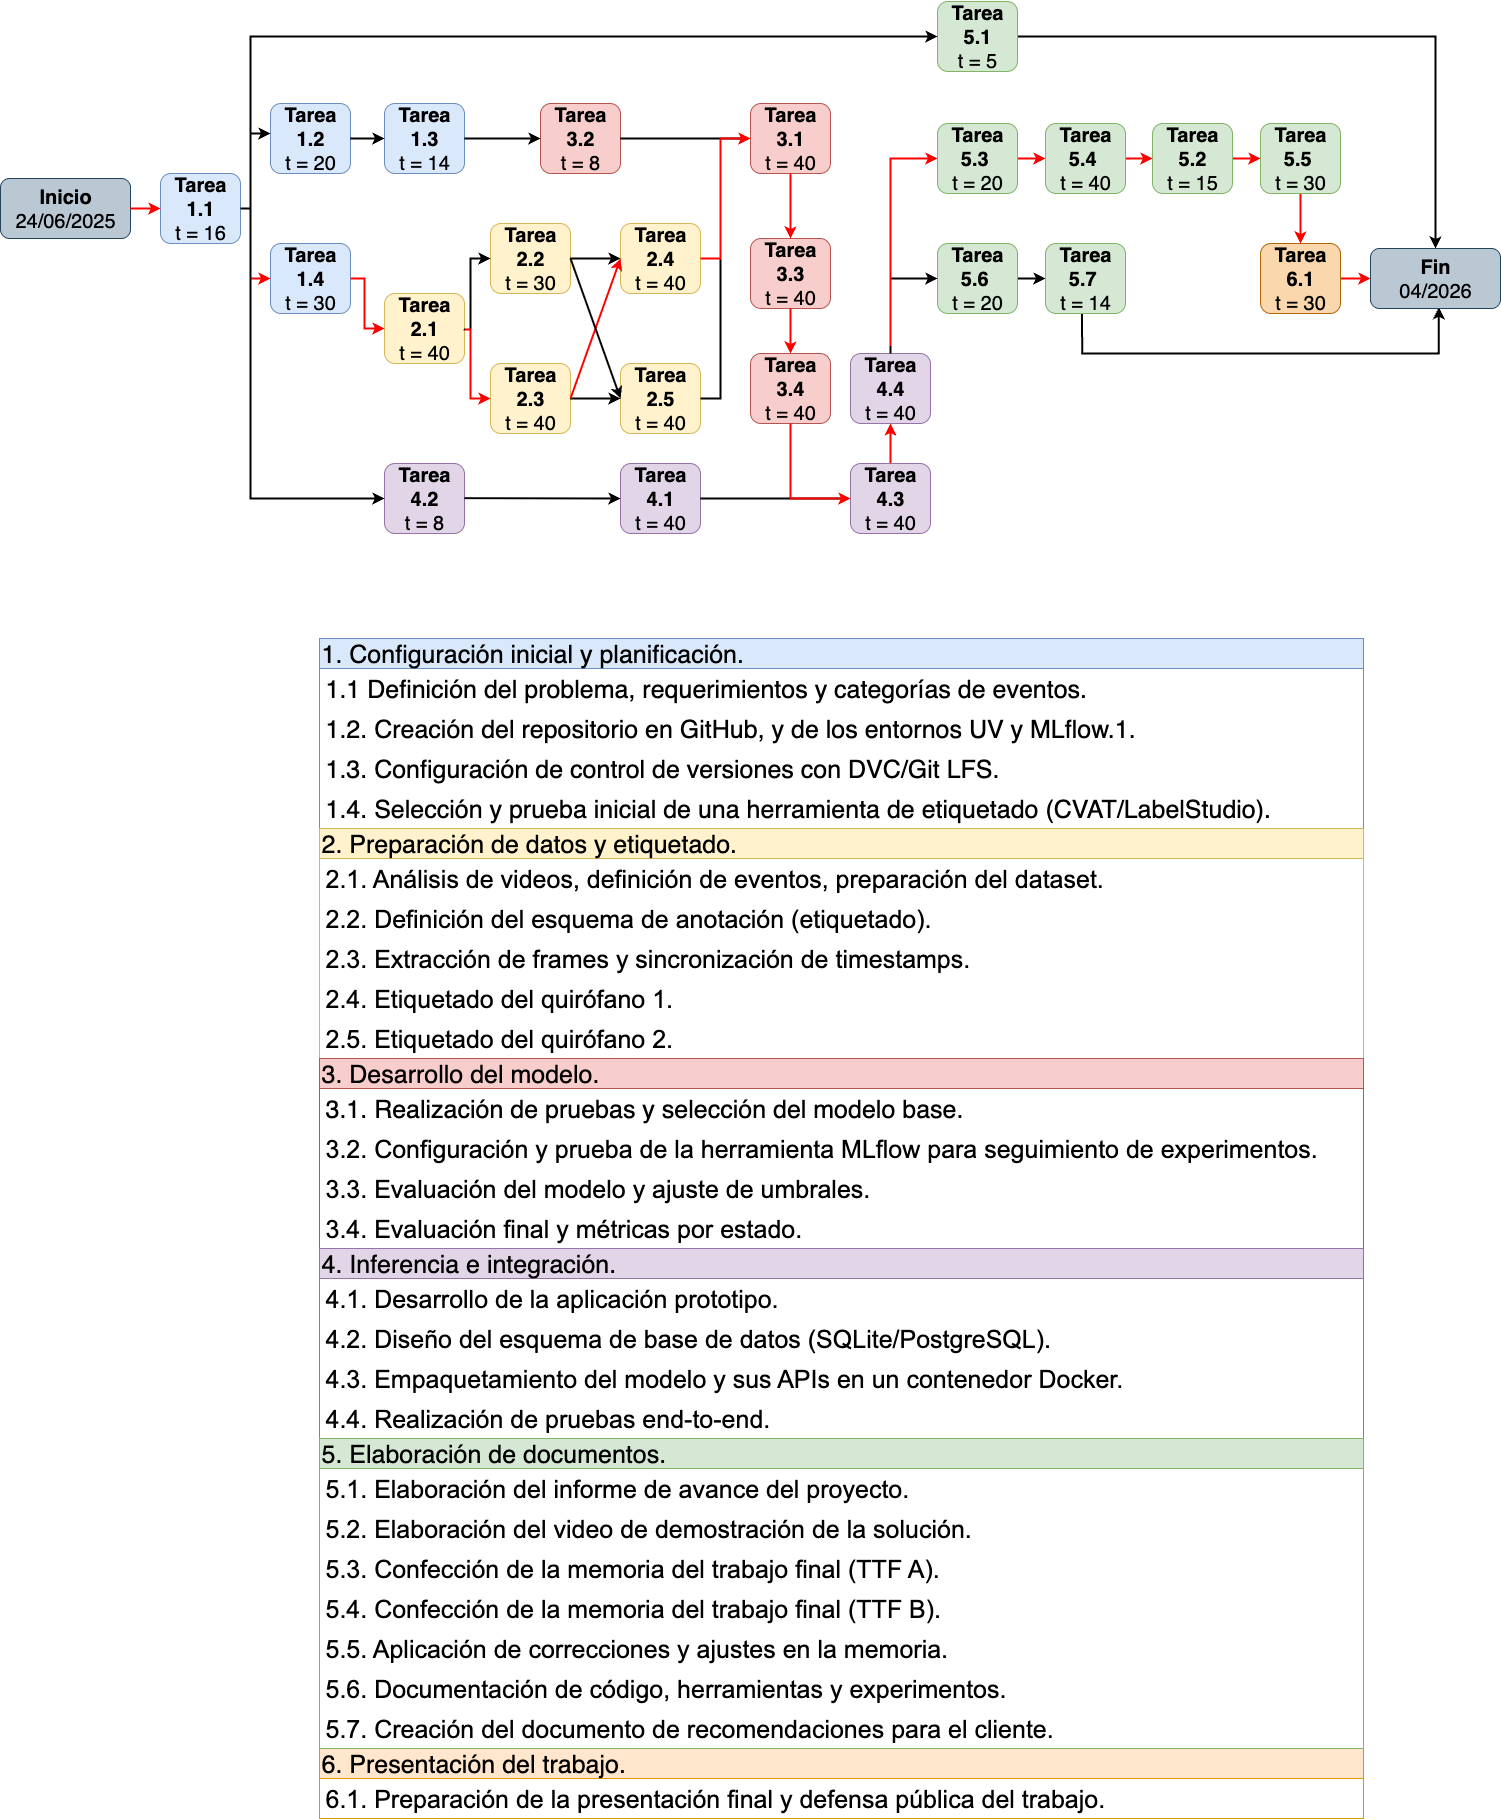
\includegraphics[width=1\textwidth]{./Figuras/CEIA-GDP-Esquema-AoN.table.png}
\caption{Diagrama de \textit{Activity on Node}.}
\label{fig:AoN}
\end{figure}



\section{11. Diagrama de Gantt}
\label{sec:gantt}

\begin{consigna}{red}
Existen muchos programas y recursos \textit{online} para hacer diagramas de Gantt, entre los cuales destacamos:

\begin{itemize}
\item Planner
\item GanttProject
\item Trello + \textit{plugins}. En el siguiente link hay un tutorial oficial: \\ \url{https://blog.trello.com/es/diagrama-de-gantt-de-un-proyecto}
\item Creately, herramienta online colaborativa. \\\url{https://creately.com/diagram/example/ieb3p3ml/LaTeX}
\item Se puede hacer en latex con el paquete \textit{pgfgantt}\\ \url{http://ctan.dcc.uchile.cl/graphics/pgf/contrib/pgfgantt/pgfgantt.pdf}
\end{itemize}

Pegar acá una captura de pantalla del diagrama de Gantt, cuidando que la letra sea suficientemente grande como para ser legible. 
Si el diagrama queda demasiado ancho, se puede pegar primero la ``tabla'' del Gantt y luego pegar la parte del diagrama de barras del diagrama de Gantt.

Configurar el software para que en la parte de la tabla muestre los códigos del EDT (WBS).\\
Configurar el software para que al lado de cada barra muestre el nombre de cada tarea.\\
Revisar que la fecha de finalización coincida con lo indicado en el Acta Constitutiva.

En la figura \ref{fig:gantt}, se muestra un ejemplo de diagrama de gantt realizado con el paquete de \textit{pgfgantt}. 
En la plantilla pueden ver el código que lo genera y usarlo de base para construir el propio.

Las fechas pueden ser calculadas utilizando alguna de las herramientas antes citadas. Sin embargo, el siguiente ejemplo
fue elaborado utilizando 
\href{https://docs.google.com/spreadsheets/d/1fBz8NhSpc4tkkhz3KjJCbh1nR_ltDkfEcZi4tZXduqs}{esta hoja de cálculo}.

Es importante destacar que el ancho del diagrama estará dado por la longitud del texto utilizado para las tareas 
(Ejemplo: tarea 1, tarea 2, etcétera) y el valor \textit{x unit}. Para mejorar la apariencia del diagrama, es necesario
ajustar este valor y, quizás, acortar los nombres de las tareas.

\begin{figure}[htpb]
  \begin{center}
    \begin{ganttchart}[
      time slot unit=day,
      time slot format=isodate,
      x unit=0.038cm,
      y unit title=0.7cm,
      y unit chart=0.6cm,
      milestone/.append style={xscale=4}
      ]{2021-03-05}{2021-12-16}
      \gantttitlecalendar*{2021-03-05}{2021-12-16}{year} \\
      \gantttitlecalendar*{2021-03-05}{2021-12-16}{month} \\
      \ganttgroup{Duración Total}{2021-03-05}{2021-12-16} \\
      %%%%%%%%%%%%%%%%%Organización
      \ganttgroup{Organización}{2021-03-05}{2021-04-16} \\
      \ganttbar{Planificación del proyecto}{2021-03-05}{2021-04-15} \\
      %%%%%%%%%%%%%%%%%Ejecución
      \ganttgroup{Ejecución}{2021-04-16}{2021-10-21} \\
      \ganttbar{Tarea 1}{2021-04-16}{2021-04-29} \\
      \ganttbar{Tarea 2}{2021-04-30}{2021-05-13} \\
      \ganttbar{Tarea 3}{2021-05-14}{2021-05-27} \\
      \ganttbar{Tarea 4}{2021-05-28}{2021-07-12} \\
      \ganttbar{Tarea 5}{2021-07-13}{2021-08-09} \\
      \ganttbar{Tarea 6}{2021-08-10}{2021-09-23} \\
      \ganttbar{Tarea 7}{2021-09-24}{2021-09-30} \\
      \ganttbar{Tarea 8}{2021-10-01}{2021-10-14} \\
      \ganttbar{Tarea 9}{2021-10-15}{2021-10-21} \\
      % %%%%%%%%%%%%%%%%%Finalización
      \ganttgroup{Finalización}{2021-10-22}{2021-12-16} \\
      \ganttbar{Memoria v1}{2021-10-22}{2021-11-04} \\
      \ganttbar{Memoria v2}{2021-11-05}{2021-11-18} \\
      \ganttbar{Memoria final}{2021-11-19}{2021-12-02} \\
      % La fecha del siguiente milestone es la fecha en que terminamos la memoria
      \ganttmilestone{Enviar memoria al director}{2021-12-02} \\
      \ganttbar{Elaborar la presentación}{2021-12-03}{2021-12-16} \\
      \ganttmilestone{Ensayo de la presentación}{2021-12-16} \\
      %%%%%%%%%%%%%%%%%%%%%%%%%%%%%%%%%%%%%%%%%%%%%%%%%%%%%%%%%%%%%%%
    \end{ganttchart}
  \end{center}
  \caption{Diagrama de gantt de ejemplo}
  \label{fig:gantt}
\end{figure}


\begin{landscape}
\begin{figure}[htpb]
\centering 
\includegraphics[height=.85\textheight]{./Figuras/Gantt-2.png}
\caption{Ejemplo de diagrama de Gantt (apaisado).} %Modificar este título acorde.
\label{fig:diagGantt}
\end{figure}

\end{landscape}

\end{consigna}


\section{12. Presupuesto detallado del proyecto}
\label{sec:presupuesto}

\begin{consigna}{red}
Si el proyecto es complejo entonces separarlo en partes:
\begin{itemize}
	\item Un total global, indicando el subtotal acumulado por cada una de las áreas.
	\item El desglose detallado del subtotal de cada una de las áreas.
\end{itemize}

IMPORTANTE: No olvidarse de considerar los COSTOS INDIRECTOS.

Incluir la aclaración de si se emplea como moneda el peso argentino (ARS) o si se usa moneda extranjera (USD, EUR, etc). Si es en moneda extranjera se debe indicar la tasa de conversión respecto a la moneda local en una fecha dada.

\end{consigna}

\begin{table}[htpb]
\centering
\begin{tabularx}{\linewidth}{@{}|X|c|r|r|@{}}
\hline
\rowcolor[HTML]{C0C0C0} 
\multicolumn{4}{|c|}{\cellcolor[HTML]{C0C0C0}COSTOS DIRECTOS} \\ \hline
\rowcolor[HTML]{C0C0C0} 
Descripción &
  \multicolumn{1}{c|}{\cellcolor[HTML]{C0C0C0}Cantidad} &
  \multicolumn{1}{c|}{\cellcolor[HTML]{C0C0C0}Valor unitario} &
  \multicolumn{1}{c|}{\cellcolor[HTML]{C0C0C0}Valor total} \\ \hline
 &
  \multicolumn{1}{c|}{} &
  \multicolumn{1}{c|}{} &
  \multicolumn{1}{c|}{} \\ \hline
 &
  \multicolumn{1}{c|}{} &
  \multicolumn{1}{c|}{} &
  \multicolumn{1}{c|}{} \\ \hline
\multicolumn{1}{|l|}{} &
   &
   &
   \\ \hline
\multicolumn{1}{|l|}{} &
   &
   &
   \\ \hline
\multicolumn{3}{|c|}{SUBTOTAL} &
  \multicolumn{1}{c|}{} \\ \hline
\rowcolor[HTML]{C0C0C0} 
\multicolumn{4}{|c|}{\cellcolor[HTML]{C0C0C0}COSTOS INDIRECTOS} \\ \hline
\rowcolor[HTML]{C0C0C0} 
Descripción &
  \multicolumn{1}{c|}{\cellcolor[HTML]{C0C0C0}Cantidad} &
  \multicolumn{1}{c|}{\cellcolor[HTML]{C0C0C0}Valor unitario} &
  \multicolumn{1}{c|}{\cellcolor[HTML]{C0C0C0}Valor total} \\ \hline
\multicolumn{1}{|l|}{} &
   &
   &
   \\ \hline
\multicolumn{1}{|l|}{} &
   &
   &
   \\ \hline
\multicolumn{1}{|l|}{} &
   &
   &
   \\ \hline
\multicolumn{3}{|c|}{SUBTOTAL} &
  \multicolumn{1}{c|}{} \\ \hline
\rowcolor[HTML]{C0C0C0}
\multicolumn{3}{|c|}{TOTAL} &
   \\ \hline
\end{tabularx}%
\end{table}


\section{13. Gestión de riesgos}
\label{sec:riesgos}

\begin{consigna}{red}
a) Identificación de los riesgos (al menos cinco) y estimación de sus consecuencias:
 
Riesgo 1: detallar el riesgo (riesgo es algo que si ocurre altera los planes previstos de forma negativa)
\begin{itemize}
	\item Severidad (S): mientras más severo, más alto es el número (usar números del 1 al 10).\\
	Justificar el motivo por el cual se asigna determinado número de severidad (S).
	\item Probabilidad de ocurrencia (O): mientras más probable, más alto es el número (usar del 1 al 10).\\
	Justificar el motivo por el cual se asigna determinado número de (O). 
\end{itemize}   

Riesgo 2:
\begin{itemize}
	\item Severidad (S): X.\\
	Justificación...
	\item Ocurrencia (O): Y.\\
	Justificación...
\end{itemize}

Riesgo 3:
\begin{itemize}
	\item Severidad (S):  X.\\
	Justificación...
	\item Ocurrencia (O): Y.\\
	Justificación...
\end{itemize}


b) Tabla de gestión de riesgos:      (El RPN se calcula como RPN=SxO)

\begin{table}[htpb]
\centering
\begin{tabularx}{\linewidth}{@{}|X|c|c|c|c|c|c|@{}}
\hline
\rowcolor[HTML]{C0C0C0} 
Riesgo & S & O & RPN & S* & O* & RPN* \\ \hline
       &   &   &     &    &    &      \\ \hline
       &   &   &     &    &    &      \\ \hline
       &   &   &     &    &    &      \\ \hline
       &   &   &     &    &    &      \\ \hline
       &   &   &     &    &    &      \\ \hline
\end{tabularx}%
\end{table}

Criterio adoptado: 

Se tomarán medidas de mitigación en los riesgos cuyos números de RPN sean mayores a...

Nota: los valores marcados con (*) en la tabla corresponden luego de haber aplicado la mitigación.

c) Plan de mitigación de los riesgos que originalmente excedían el RPN máximo establecido:
 
Riesgo 1: plan de mitigación (si por el RPN fuera necesario elaborar un plan de mitigación).
  Nueva asignación de S y O, con su respectiva justificación:
  \begin{itemize}
	\item Severidad (S*): mientras más severo, más alto es el número (usar números del 1 al 10).
          Justificar el motivo por el cual se asigna determinado número de severidad (S).
	\item Probabilidad de ocurrencia (O*): mientras más probable, más alto es el número (usar del 1 al 10).
          Justificar el motivo por el cual se asigna determinado número de (O).
	\end{itemize}

Riesgo 2: plan de mitigación (si por el RPN fuera necesario elaborar un plan de mitigación).
 
Riesgo 3: plan de mitigación (si por el RPN fuera necesario elaborar un plan de mitigación).

\end{consigna}


\section{14. Gestión de la calidad}
\label{sec:calidad}

\begin{consigna}{red}
Elija al menos diez requerimientos que a su criterio sean los más importantes/críticos/que aportan más valor y para cada uno de ellos indique las acciones de verificación y validación que permitan asegurar su cumplimiento.

\begin{itemize} 
\item Req \#1: copiar acá el requerimiento con su correspondiente número.

\begin{itemize}
	\item Verificación para confirmar si se cumplió con lo requerido antes de mostrar el sistema al cliente. Detallar.
	\item Validación con el cliente para confirmar que está de acuerdo en que se cumplió con lo requerido. Detallar. 
\end{itemize}

\end{itemize}

Tener en cuenta que en este contexto se pueden mencionar simulaciones, cálculos, revisión de hojas de datos, consulta con expertos, mediciones, etc.  

Las acciones de verificación suelen considerar al entregable como ``caja blanca'', es decir se conoce en profundidad su funcionamiento interno.  

En cambio, las acciones de validación suelen considerar al entregable como ``caja negra'', es decir, que no se conocen los detalles de su funcionamiento interno.

\end{consigna}

\section{15. Procesos de cierre}    
\label{sec:cierre}

\begin{consigna}{red}
Establecer las pautas de trabajo para realizar una reunión final de evaluación del proyecto, tal que contemple las siguientes actividades:

\begin{itemize}
	\item Pautas de trabajo que se seguirán para analizar si se respetó el Plan de Proyecto original:\\
	 - Indicar quién se ocupará de hacer esto y cuál será el procedimiento a aplicar. 
	\item Identificación de las técnicas y procedimientos útiles e inútiles que se emplearon, los problemas que surgieron y cómo se solucionaron:\\
	 - Indicar quién se ocupará de hacer esto y cuál será el procedimiento para dejar registro.
	\item Indicar quién organizará el acto de agradecimiento a todos los interesados, y en especial al equipo de trabajo y colaboradores:\\
	  - Indicar esto y quién financiará los gastos correspondientes.
\end{itemize}

\end{consigna}

\end{document}